\subsection{Certified prefix transfer and a finite resolution threshold}
\label{ssec:certified-prefix-transfer}

The joint update can be evaluated for every prefix without solving a
new eigenproblem at each $N$. Write $x_j=j^2$ and
$A_{ij}=(r_iw_j-w_ir_j)/(x_i-x_j)$, with original leading functional
$w=(1,\sqrt2,\ldots)^T$. Let $\widetilde r_j,\widetilde w_j,d_j$
be the generators and positive pivot when natural-order LDL elimination
reaches index $j$. Starting with $R_{-1}=1,W_{-1}=0$, define, away from
the Fourier nodes,
\[
 c_j(t)=\frac{R_{j-1}(t)\widetilde w_j-W_{j-1}(t)\widetilde r_j}{t-x_j},
 \qquad
 \binom{R_j}{W_j}=\binom{R_{j-1}}{W_{j-1}}
       -\frac{c_j}{d_j}\binom{\widetilde r_j}{\widetilde w_j}.
\]
If $c(t)_j=w_j/(t-x_j)$ uses the original generators, elimination gives
\[
 R_N=1-c(t)^TA_N^{-1}r,\quad W_N=-c(t)^TA_N^{-1}w,
 \quad H_N=w^TA_N^{-1}w=\sum_{j=0}^N\frac{\widetilde w_j^2}{d_j}.
\]
Thus the monic transform is
\[
 F_N(\nu)=-\frac{2\sin(\nu L/2)}{\sqrt L}
               \frac{\nu}{\beta^2 H_N}W_N((\nu/\beta)^2).
\]
Node limits must be taken separately. One $O(M^2)$ factorization and
one $O(M)$ transfer per evaluation point provide all $N\le M$.
Direct expansion of the determinant-one update also proves
\[
 \frac{R_N(t)W_N(u)-W_N(t)R_N(u)}{u-t}
       =\sum_{j=0}^N\frac{c_j(t)c_j(u)}{d_j},\qquad
 R_NW_N'-W_NR_N'=\sum_{j=0}^N\frac{c_j(t)^2}{d_j}>0.
\]
This positive derivative kernel supplies a local root tool, but poles
of $R_N$ must still be checked; positivity does not justify Newton
iteration across one of them.

\begin{proposition}[Ordinal counts and nested zero-shift interlacing]
\label{prop:prefix-count-interlacing}
Let $A_M>0$ be a consistent finite source, $D=\operatorname{diag}(x_j)$,
and $S=A_MD+rw^T=DA_M+wr^T$. The degree-$N$ monic squared roots are
the generalized eigenvalues of $(J_N^TS_NJ_N,J_N^TA_NJ_N)$, where
$J_N=[-w_{1:N}^T;I_N]$. Away from nodes and zero leading pivots,
\[
 Z_N(t)=\frac{W_N(t)}{R_N(t)}=w^T(S_N-tA_N)^{-1}w,
 \qquad
 \#\{\theta_{j,N}<t\}=n_-(S_N-tA_N)+\boldsymbol1_{\{Z_N(t)>0\}}-1.
\]
The full-pencil negative count is obtained from the signs of
$d_j(x_j-t)R_j/R_{j-1}$. Moreover,
\[
 \theta_{k,N+1}\le\theta_{k,N}\le\theta_{k+1,N+1},\qquad 1\le k\le N.
\]
\end{proposition}
\begin{proof}
The compressed-pencil representation is the finite monic variational
identity. The determinant identity
$\det(S_j-tA_j)=\det(A_j)\prod_{i=0}^j(x_i-t)R_j(t)$ gives the pivot
signs. The bordered matrix with blocks $S_N-tA_N,w,w^T,0$ has the
inertia of $S_N-tA_N$ plus the sign of $-Z_N$. Compression to
$\ker w^T$ instead leaves one positive and one negative direction;
equating negative counts proves the count formula. Finally, the spaces
\[
 V_N=\{v\in\mathbb R^{M+1}:v_j=0\ (j>N),\ w^Tv=0\}
\]
are nested and have dimension $N$. All their Ritz values concern the
same pair $(S,A_M)$. The min--max principle proves interlacing.
\end{proof}

An unresolved interval sign is an unresolved count, not a rounded
decision. The transfer and inertia identities pass 7290 and 5292 exact
rational checks on 30 positive fixtures each. A separate streaming and
nested-compression check passes 3328 checks on 52 fixtures.

\paragraph{Transfer to the analytic source.}
Positive rounded factors define a precise surrogate, denoted by hats.
Its roots alone do not certify the analytic matrix. Put
$H=J^TAJ$, $T=J^TSJ$ and suppose
\[
 \widehat H\succeq gI,\quad
 \|H-\widehat H\|\le E_H,\quad
 \|T-\widehat T\|\le E_T,\quad e=E_H/g<1,\quad f=E_T/g.
\]
If the lowest surrogate squared root exceeds $f$, Loewner bounds and
min--max give, with the same index,
\[
 \frac{\widehat\theta_k-f}{1+e}\le\theta_k
             \le\frac{\widehat\theta_k+f}{1-e}.
\]
Here the bounds include both the matrix generators and the perturbed
leading functional. Interval reconstruction of the natural factors,
an inverse-trace lower bound, and the existing analytic generator
enclosures establish these hypotheses for the $C=125,M=2000$ source
and all its prefixes. A baseline count at $\nu=0.1$ verifies positivity
for every prefix. For $\widehat\theta_k\le2\times10^6$, the resulting
frequency motion is at most $3.184\times10^{-1458}$. Consequently the
following error intervals concern the finite \emph{analytic zero-shift}
pencil, including the reference-zero uncertainty.

\begin{center}
\begin{tabular}{rrrr}
\toprule
$N$ & matched prefix & $D^{(0)}_1$ & $D^{(0)}_{1000}$ \\
\midrule
1000 & 902 & $[656.2556,656.2565]$ & unmatched \\
1250 & 1000 & $[666.7057,666.7067]$ & $[22.1208,22.1218]$ \\
1500 & 1000 & $[666.8629,666.8639]$ & $[22.3172,22.3182]$ \\
1750 & 1000 & $[666.9341,666.9350]$ & $[22.3718,22.3728]$ \\
2000 & 1000 & $[666.9774,666.9784]$ & $[22.3993,22.4003]$ \\
\bottomrule
\end{tabular}
\end{center}
Here $D^{(0)}_k=-\log_{10}|(\nu^{(0)}_{k,N}-\gamma_k)/\gamma_k|$.
All 5000 requested pairs are retained: 4902 have certified error
brackets; the other 98 are proved above their reference windows.
Three initial linearization brackets at $N=1000$, $k=900,901,902$
failed despite window membership and were refined by count bisection.
The initial arithmetic attempt with full reference balls was also
unresolved and is retained. Qualified point evaluations separate the
reference radius, use 2300 or 3500 decimal working digits, and are
followed by ordinal and source checks. The source certificate uses
6000 decimal working digits. These are working precisions, not a
minimum-bit-$P$ theorem.

\paragraph{A measured minimum mode budget.}
Guarded counts at the reference midpoint boundaries classify every
integer $N=1,\ldots,2000$ and $k=1,\ldots,1000$: two million dependent
target pairs from the same source. Both guard endpoints use a fixed
$10^{-6}$ frequency margin; the pencil inequalities certify that their
equal counts persist at the analytic midpoint. No count is unresolved.
The first complete 1000-target window match occurs at $N=1091$;
$N=1090$ matches only 999. All individual matches persist through
$N=2000$. This is a window-resolution threshold, not a specified
digit-accuracy threshold or a statement about larger $N$.

The previously derived, unfitted continuum turning-point budget is
\[
 N_{\rm turn}(C,x)=\frac{x\ell_x}{4}\frac{\sin u_x}{u_x},\qquad
 \ell_x=\log\frac{x}{4\pi},\qquad
 u_x=\frac{\pi\ell_x}{2\log C},\qquad 4\pi<x<4\pi C.
\]
At $x=\gamma_k$ it has 1.653 modes RMS discrepancy from the 1000
individual entry thresholds. It predicts $1090.163$ for $k=1000$,
whose actual threshold is 1091. Yet
$\max\{k,\lceil N_{\rm turn}\rceil\}$ is insufficient at 249 indices,
by as many as six modes. Its closeness cannot be promoted to a sufficient
CCM budget; neither can an empirical six-mode padding be declared
uniform. Reference heights here assess a model, not a reference-free
zero predictor.

\begin{figure}[htbp]
\centering
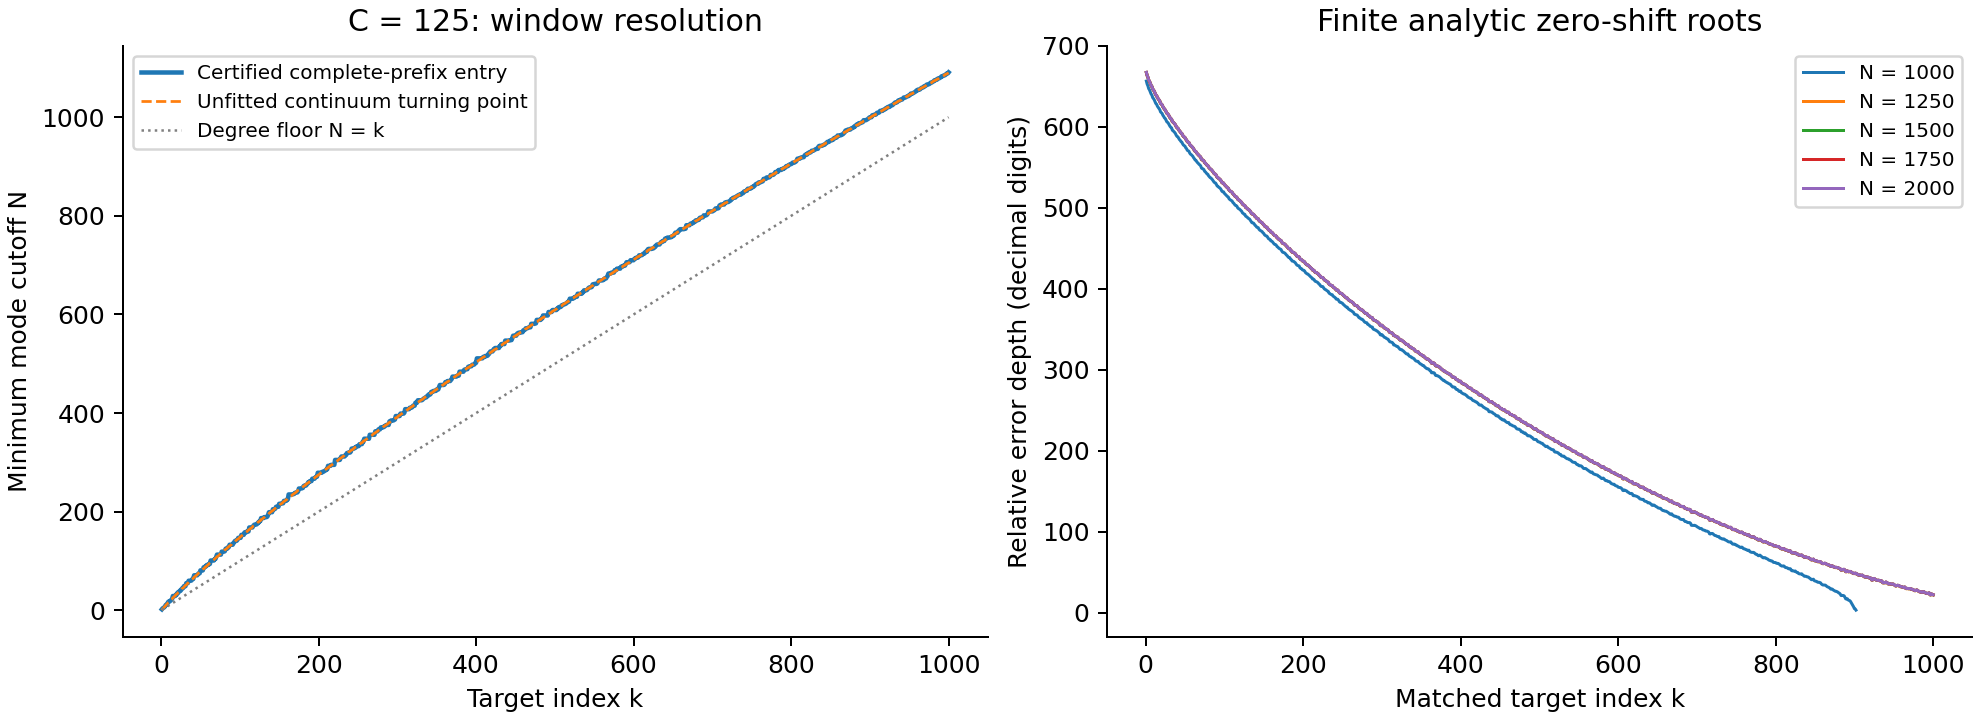
\includegraphics[width=\linewidth]{figures/prefix_resolution.png}
\caption{Certified zero-shift resolution and errors at $C=125$.
The continuum threshold closely tracks the finite entry curve but
fails as a sufficient integer budget. The $N=1000$ error curve ends
at its last matched target, $k=902$; no unmatched value is scored.}
\label{fig:prefix-resolution}
\end{figure}

For a fixed upper boundary $b_k$, interlacing makes
$N_{\rm entry}=\min\{N\ge k:\#(\nu_{j,N}^{(0)}<b_k)\ge k\}$
a monotone entry event. A lower-boundary count is also needed: a root
could later leave its window downward. Replacing the window by
$\gamma_k(1\pm10^{-d})$ provides a count-based finite $d$-digit test.
The desired law therefore needs a resolution gate before combining
physical, ground-source and arithmetic error budgets. For established
upper bounds $E_R,E_G,E_P$, the triangle inequality gives
\[
 D_{\rm total}\ge-\log_{10}(E_R+E_G+E_P)
       \ge\min\{D_R,D_G,D_P\}-\log_{10}3.
\]
This is a conditional bound, not an equality or a fitted rate.
Uniform parameter bounds for its channels remain open. In particular,
zero-shift interlacing and source certification do not certify the
changing ground-transform root errors or identify the infinite-cutoff
limit with the zeta zeros.
